\section{Auswertung}

Ausgleichsrechnungen mit Fehlerfortpflanzung werden mit scipy.curve\_fit aus dem Programm Python
durchgeführt.

\subsection{Kontrast}

Fit nach der Funktion
\[
K = a \cdot | \sin (2 \cdot \phi + b) |
\]
liefert Fitparameter $a = 1.06 \pm 0.05$ und $b = 1 \pm 2$

\begin{figure}[h]
\centering
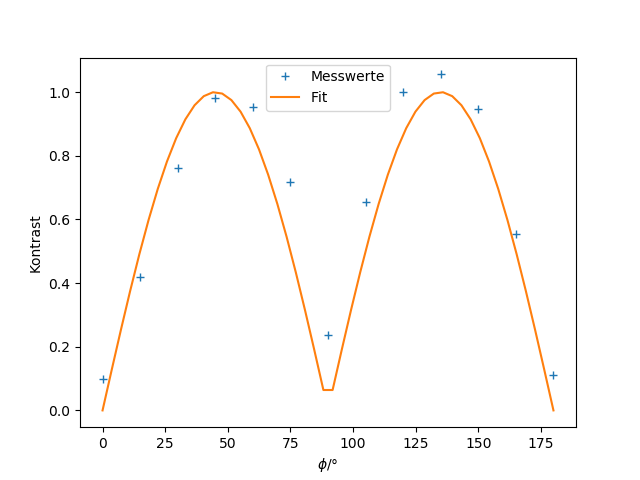
\includegraphics[width=\linewidth]{img/kontrast.png}
\caption{Ausgleichsrechnung für den Zusammenhang zwischen dem Winkel $\phi$ und dem Kontrast $K$.}
\label{kontrast}
\end{figure}

\subsection{Brechungsindex von Glas}

Fit nach der Funktion
\[
N = a \cdot \theta + b
\]
liefert Fitparameter $a = 3.36 \pm 0.09$ und $b = 0.8 \pm 0.6$

\begin{figure}[h]
\centering
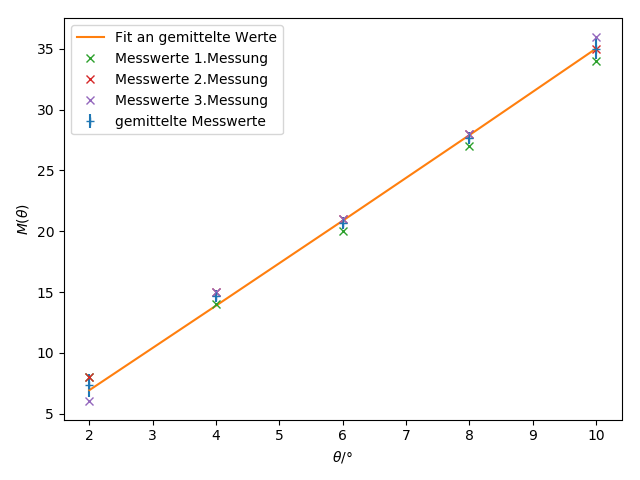
\includegraphics[width=\linewidth]{img/n_glas.png}
\caption{Lineare Ausgleichsrechnung für den Zusammenhang zwischen dem Winkel $\theta$ und der Anzahl
der Intensitätsmaxima.}
\label{n_glas}
\end{figure}

\subsection{Brechungsindex von Luft}

Fit nach der Funktion
\[
N = a \cdot p + b
\]
liefert Fitparameter $a = 0.0478 \pm 0.0008$ und $b = -0.4 \pm 0.2$

\begin{figure}[h]
\centering
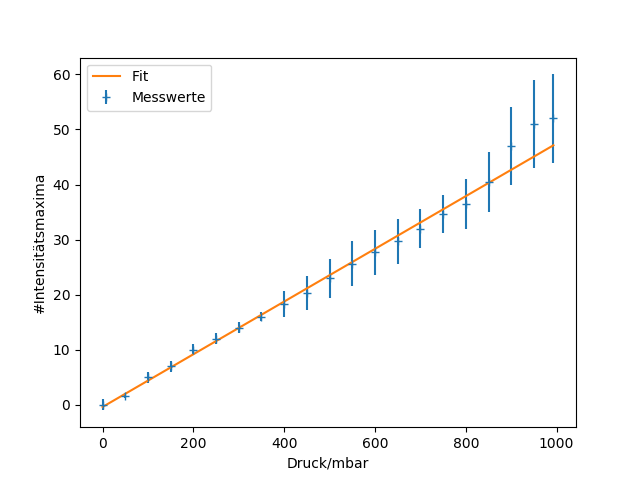
\includegraphics[width=\linewidth]{img/n_luft.png}
\caption{Lineare Ausgleichsrechnung für den Zusammenhang zwischen dem Druck $p$ und der Anzahl
der Intensitätsmaxima.}
\label{n_luft}
\end{figure}
